\documentclass{mylib/reporteConCalif}
\usepackage{float}

\title{Reporte}
\author{rodrigofranciscopablo }

\subject{Laboratorio de Diseño Digital}
\mytitle{Reporte de práctica 5}
\mysubTitle{Minimización de funciones por mapas de Karnahugh}
\students{Francisco Pablo \textsc{Rodrigo}}
\teacher{M.I. Guevara Rodríguez \textsc{Ma. del Socorro}}
\group{6}
\deliverDate{18 de marzo de 2019}


\begin{document}

\coverPage

\tableofcontents
\newpage

\section{Objetivos}

\subsection{General}

El alumno diseñará circuitos combinacionales.

\subsection{Particular}

El alumno analizará, diseñará e implementará multifunciones, con funciones no especificadas,
optimizando las funciones por medio de mapas de karnahugh.

\section{Introducción}

Un mapa de Karnaugh (también conocido como tabla de Karnaugh o diagrama de Veitch, abreviado como Mapa-K o Mapa-KV) es un diagrama utilizado para la simplificación de funciones algebraicas Booleanas. El mapa de Karnaugh fue inventado en 1953 por Maurice Karnaugh, un físico y matemático de los laboratorios Bell.

El mapa de Karnaugh consiste en una representación bidimensional de la tabla de verdad de la función a simplificar. Puesto que la tabla de verdad de una función de N variables posee 2N filas, el mapa K correspondiente debe poseer también 2N cuadrados. Las variables de la expresión son ordenadas en función de su peso y siguiendo el código Gray, de manera que sólo una de las variables varía entre celdas adyacentes. 

El mapa de Karnaugh se va completando colocando los unos “1” en la celda apropiada, ayudados por la tabla de verdad. Esta agrupación
es conocida como minitérminos o minterms y como expresión booleana viene a ser una suma de productos. Usualmente no se escriben los ceros
“0” en la tabla, ya que solo se agrupan los unos “1”.

\begin{figure}[H]
	\centering
	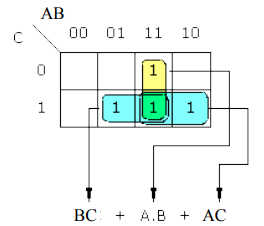
\includegraphics[width=8cm]{img/labdise_pract5/mapa-kv}
	\caption{Mapa de Karnaugh para una función de tres variables.}
\end{figure}

\newpage
\section{Previo}

\newpage
\section{Desarrollo}

Para realizar un circuito elevador de 3 bits al cuadrado recurrimos al diseño lógico de Xilinx utilizando la sección de código que a mi parecer es más sencillo que arrastrar los componentes, finalemente el código quedó de la siguiente manera.\\

\begin{center}
	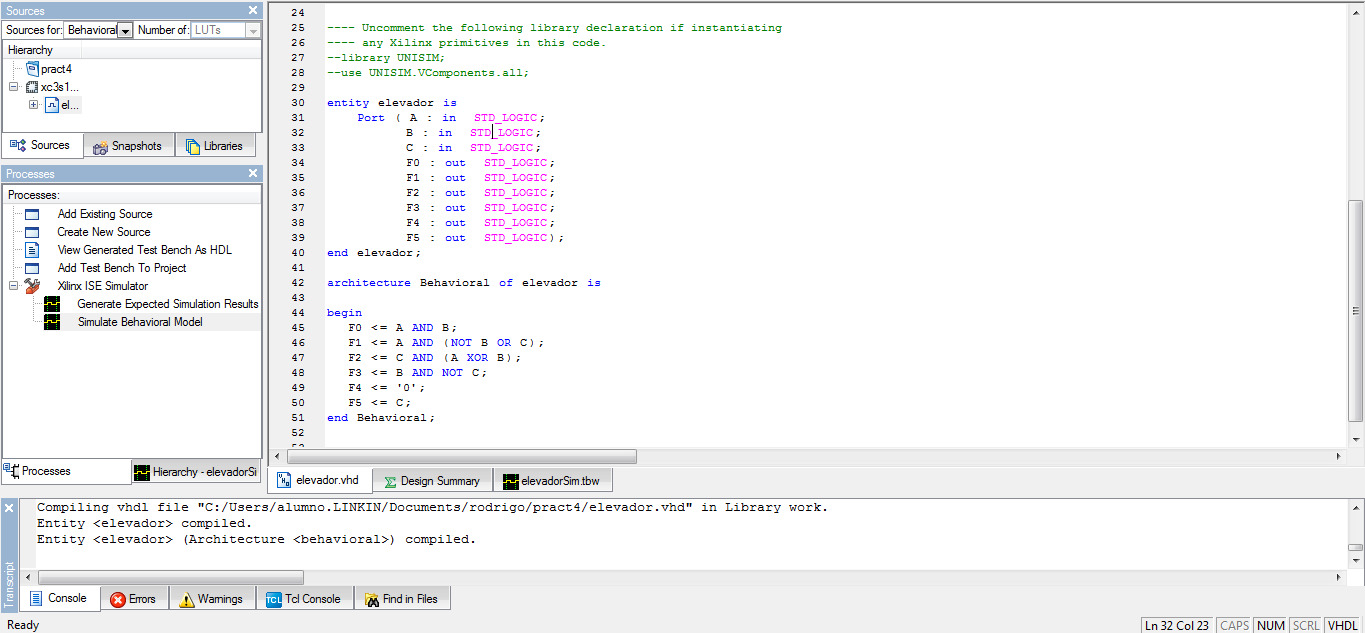
\includegraphics[width=15cm]{img/labdise_pract4/r4_img1}
\end{center}

Comprobamos que el circuito estuviera bien y para ello realizamos la simulación y probamos para diferentes valores como puede verse a continuación.\\

$000^2 = 00000$
\begin{figure}[H]
	\centering
	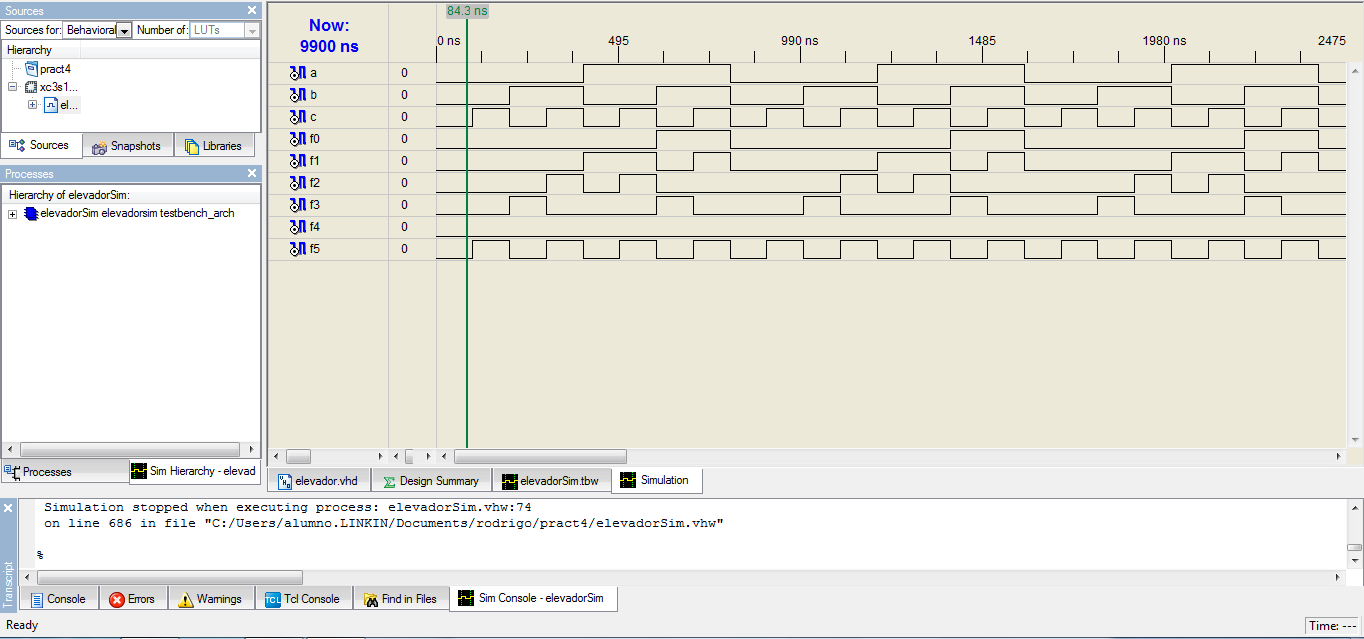
\includegraphics[width=15cm]{img/labdise_pract4/r4_img2}
	\caption{Puede verse que aquí estamos elevando cero al cuadrado y el resultado es cero.}
\end{figure}

$001^2 = 000001$
\begin{figure}[H]
	\centering
	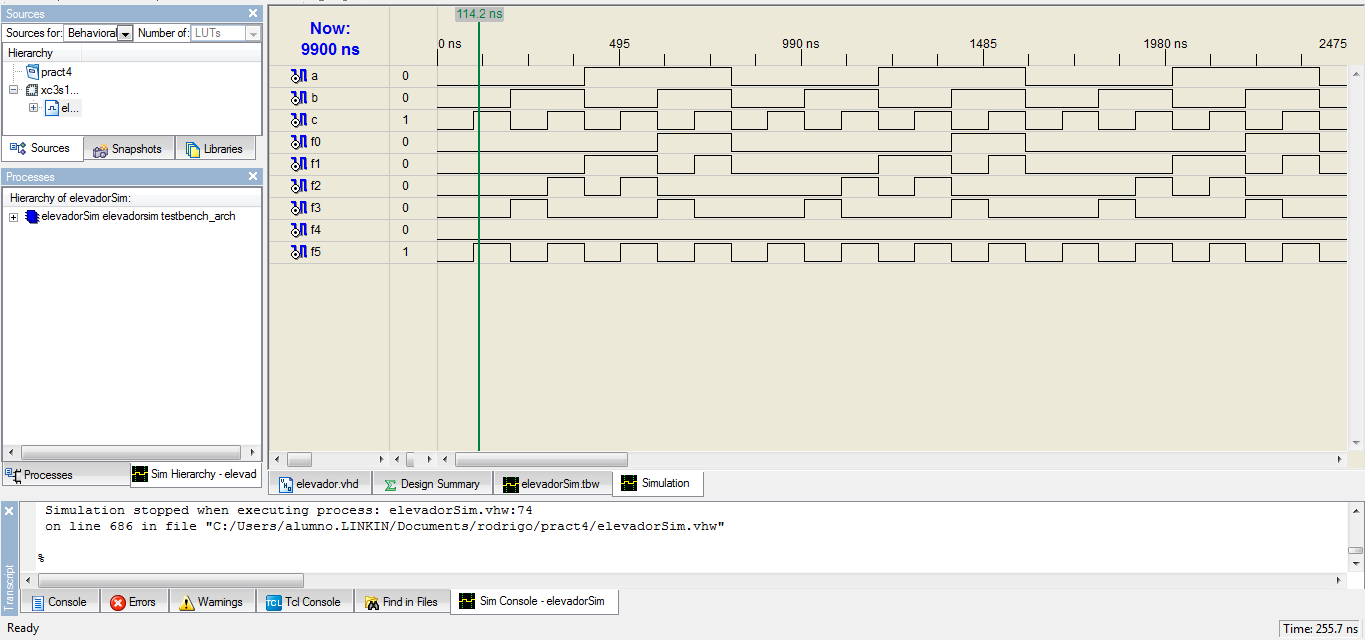
\includegraphics[width=15cm]{img/labdise_pract4/r4_img3}
	\caption{Puede verse que aquí estamos elevando uno al cuadrado y el resultado es uno.}
\end{figure}

$111^2 = 110001$
\begin{figure}[H]
	\centering
	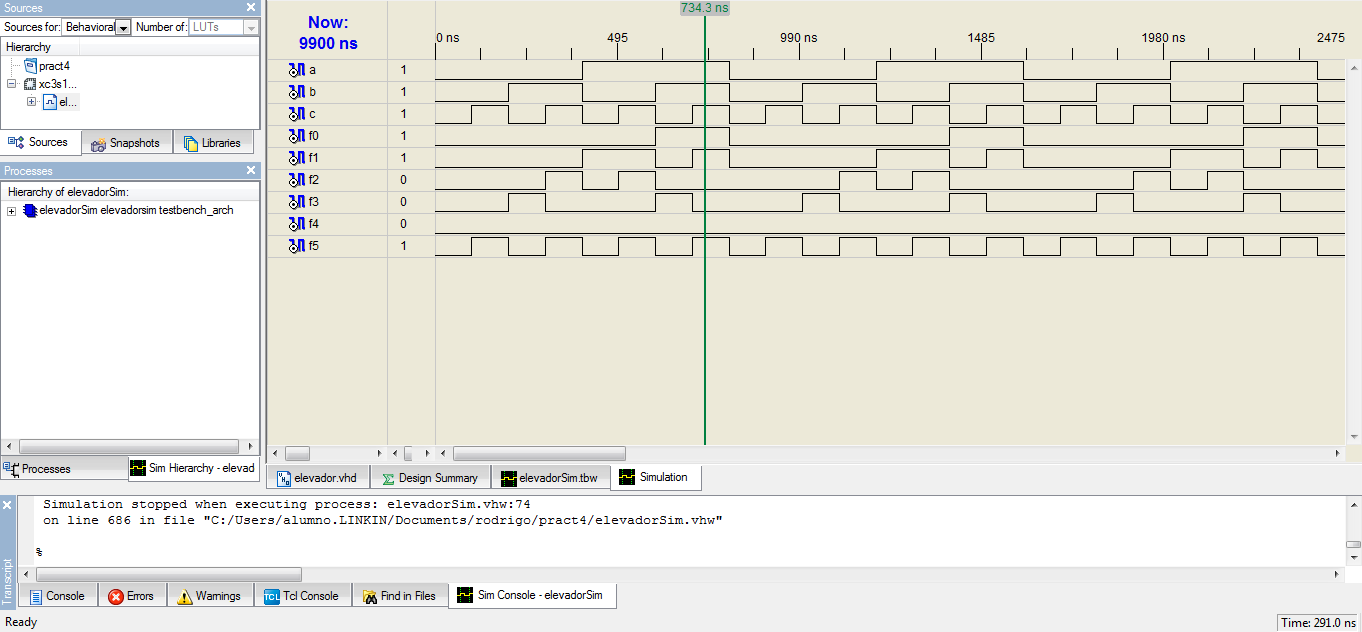
\includegraphics[width=15cm]{img/labdise_pract4/r4_img4}
	\caption{Puede verse que aquí estamos elevando siete al cuadrado y el resultado es 49.}
\end{figure}

Luego de que la fase de simulación fue exitosa pasamos nuestro diseño a la \textit{Basys2} para ello tuvimos que generar un archivo con extensión \textit{.bit} y posteriormente mediante una programa llamado \textbf{Adapt} logramos pasar nuestro circuito a la FPGA.

%Inserta imagen aqui

En la siguiente imagen se puede apreciar a nuestro dieño en funcionamiento. Utilizamos los primeros 6 LEDs y los primeros 3 switches.


\section{Conclusiones}

Al realizar el diseño del circuito identifique la importancia de saber minimizar con mapas de Karnaugh ya que sino lo hubiera hecho, el número de compuertas a utilizar sería muchisimo más grande que el que ya tenemos.\\

Se puede notar que para construir un circuito combinacional que solo puede multiplicar hasta el 7 en decimal o hasta el 111 en binario se llevo 8 compuertas (4 ANDs, 2 NOT, 1 OR y 1 XOR). Quiere decir que para hacer una multitplicación de n por n tendremos que tener muchisimas compuertas, lo cual no es optimo.\\

Por otra parte, al utilizar el modo de programación del Xilinx observe que es más rápido hacerlo de esa manera en lugar de ir arrastrando componentes y tener unirlos con cuidado.

\end{document}